\documentclass[10pt]{article}
\usepackage{amssymb, amsmath, graphicx, float, subfig, fancyhdr}


\title{Mixture Optimization Reparametrization}
\author{Nathan Willey}
\date{June 2022}

\fancypagestyle{logo}{
\fancyhf{}
\fancyhead[LE,LO]{
\includegraphics[scale=.3]{../MTRI_logo.pdf}}}
\pagestyle{logo}

\graphicspath{{./figures/}}

\begin{document}

\maketitle

\tableofcontents
\newpage 

\section{Method}

\subsection{Problem Description}
Let $f(x_1, x_2, \dots, x_N)$ be an objective function and $\{x_1, x_2, \dots, x_N\} \in \mathcal{S}_N$ where $S_N := \{\{x_1, x_2, \dots, x_N\} | \sum_{i=1}^N x_i = 1, x_i \geq 0 \ \forall i\}$. Our problem pertains to finding a well-conditioned reparametrization of such functions over the standard simplex that leads to faster, and better behaved minimization routines. \\

$\mathcal{S}_N$ is a degree $N-1$ sub-manifold with corners, and we can parameterize it with spherical coordinates $\{ \alpha_1, \alpha_2, \dots, \alpha_{N-1}\}$ using the map $M(\vec{\alpha})^2$ where $M$ is the typical map from spherical to Cartesian coordinates with an implied radius of 1. \\ We can then utilize a map $T: \mathcal{S}_N \to \mathcal{S}_N$ over the simplex defined such that each $T_i$ is a function only of $M(\vec{\alpha})^2_i$. Our goal is to map the point of isometry of the map $M(\vec{\alpha})^2: \mathbb{R}^{N-1} \to \mathcal{S}_N$ to the optima of our objective function $f$ such that our reparametrization is well-conditioned around the true solution.\\ Otherwise put, we optimally hope that $f(T(M(\vec{\alpha_{\text{isom}}})^2)) \approx x_{\text{optima}}$\\ 

\textbf{Notation: } \\ $\vec{\alpha}$- point in spherical parametrization space \\  
$\vec{y} := M(\vec{\alpha})^2$- Cartesian representation of point on the simplex. \\
\textbf{y} - Denotes the space of parameters reached by mapping spherical coordinates onto the simplex, and thus the cartesian representation of the space seen by the \textit{minimizer}\\
$\vec{x} := T(\vec{y})$- re-mapped coordinate on the simplex. \\
\textbf{x} - Denotes the parameter space reached by remapping y; Space seen by the \textit{objective function}\\

\begin{figure}[h]
	\centering
	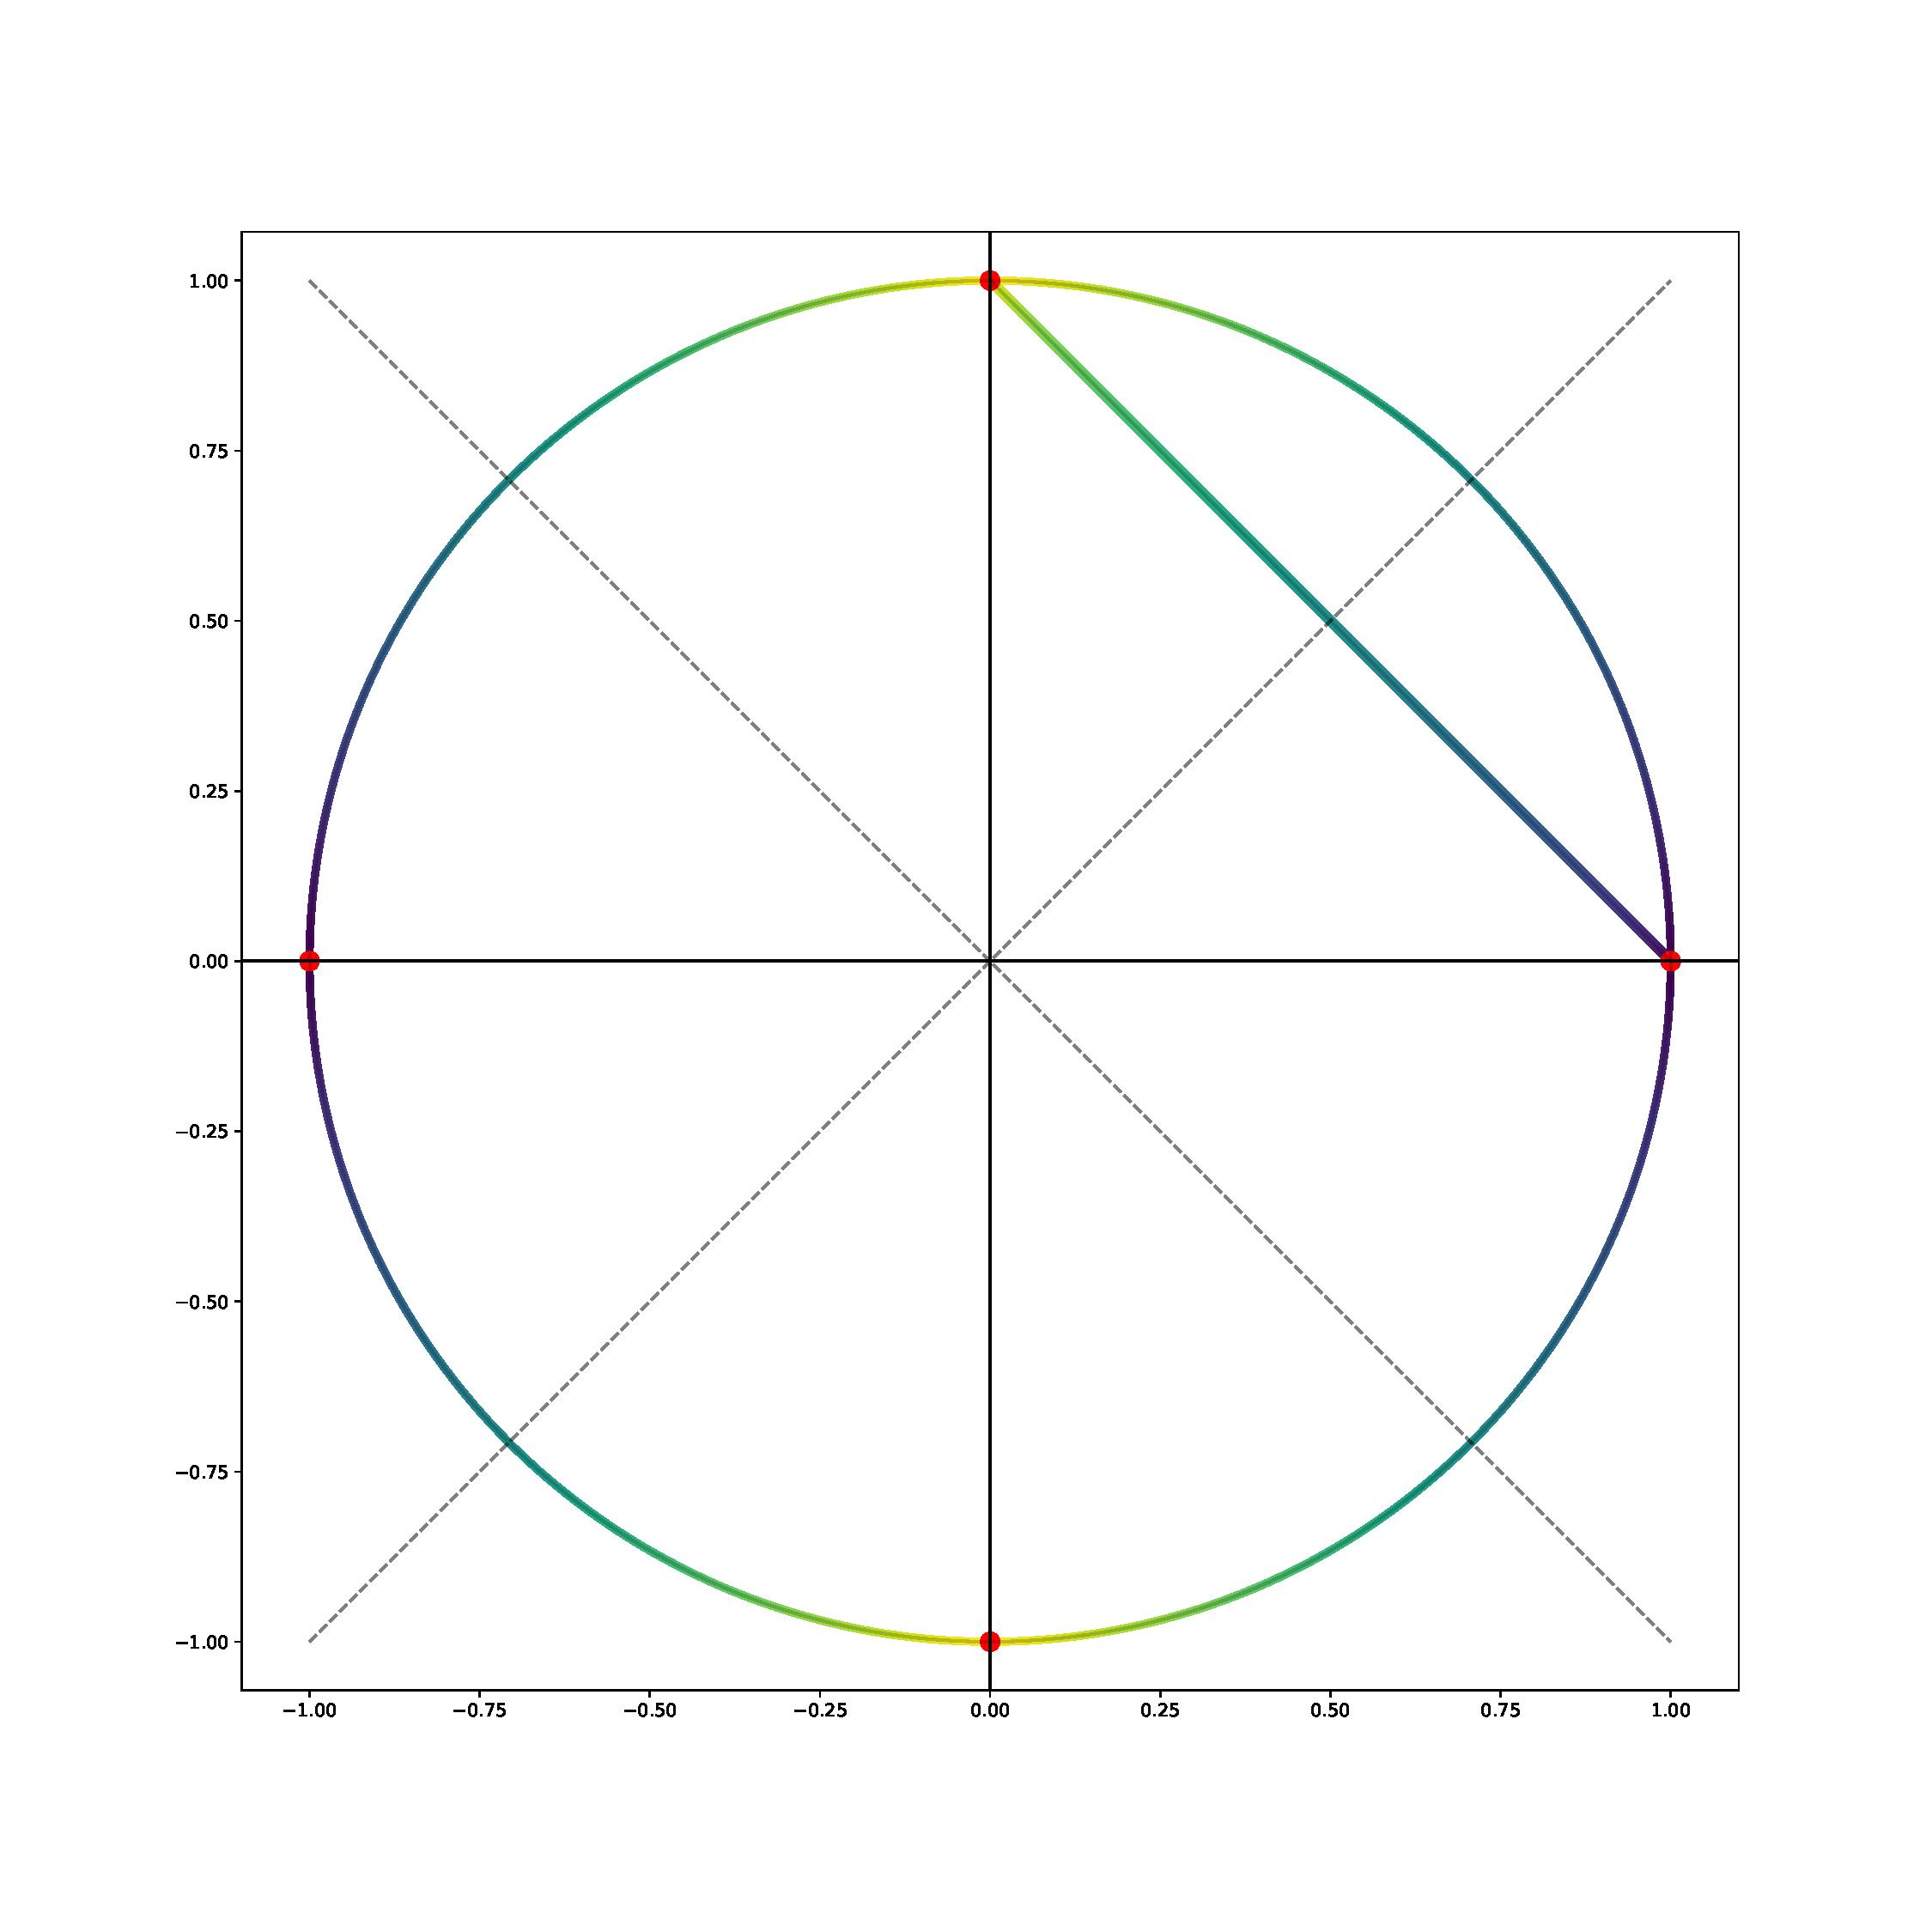
\includegraphics[width=7cm]{simplexParam.pdf}
	\caption{2D mapping from the sphere onto the simplex. Point-mapping denoted by the colormap, isometry regions are along the gray dotted lines, and the points of "non-differentiability" are shown in red.}
\end{figure}


\subsection{Choosing $T$}
A naive way to define $T$ would be to simply shift $\vec{y}$ by some vector $\beta$ s.t. $y_{\text{isom}} + \beta = x_{\text{optima}}$. The clear problem with this mapping is that it does not remain on the simplex. As such, any minimization routine utilizing it may find itself taking steps in disallowed parameter space.\\

The current approach for choice of $T$ is to use element-wise Padé splines to map directly on the simplex. The Padé splines give direct control of a "control point" which we use to map $(y_{\text{isom}})_i$ to our guess of $(x_{\text{optima}})_i$ with smooth first and second derivatives. 


\subsection{Choosing $T(y_\text{isom})$}\label{choosingRemap}

It is a given to the problem that we don't know the local optima $x_{\text{optima}}$, so we must choose a method of mapping $y_{\text{isom}}$ that guarantees that we map the point of isometry near the optima in order to have a near isometric map over which to optimize $\vec{\alpha}$. Here I outline two such possible methods. It remains to be seen how these methods compare in time and accuracy in action, and both a require more formal exploration into their convergence behavior.

\subsubsection{Re-mapping Based on Jacobian's Condition Number}\label{kappaTrack}

Quasi-Newton/Newton methods for minimization utilize a quadratic approximation to the objective function $f(x)$. We can measure a function's deviation from a quadratic using the condition number of its Jacobian $J$, in turn giving a measure of expected minimizer performance. In a general setting, we have no control over the objective function's Jacobian, but we \textit{can} track the Jacobian of our transformation from spherical coordinates onto the simplex as $J_\alpha$. 

We can use this measure on our map $\vec{\alpha} \to \vec{x}$ to determine when the mapping is too poorly conditioned. When it is, we can choose to interrupt our minimization routine and remap the isometry point s.t. $T(y_{\text{isom}}) = x_{i}$, where $x_{i}$ is the Cartesian representation of the minimizer's current step. In this way, we can improve the conditioning of the spherical-to-simplex mapping at this step as measured by the Jacobian's condition number $\kappa(J_\alpha) \equiv \kappa(J[T(M(\vec{\alpha})^2])$. 


\subsubsection{Continuous Re-mapping}\label{contRemap}

The core idea of this method is mapping $T(y_{\text{isom}}) = y_{i}$ at every kth iteration of the minimization routine. In this setup, the routine always starts the minimization step at $\alpha_{\text{isom}}$ (which maps to $x_{i}$ through $T(M(\alpha)^2)$) and searches for the best step in spherical coordinates to minimize $f$. \\ Through this process and using a minimization routine that guarantees non-increasing steps, $T$ will map closer to the true optima on each remapping, and allowing us to always be searching $\alpha$-space near the isometry point. \\ 


\newpage
\subsection{Mappings and Propagated Gradient}

It is important for minimization routines to know the gradient of the objective function with respect to the re-mapping $T$ and parametrization with $\vec{\alpha}$. Here I log the gradient of the objective function with respect to $\vec{\alpha}$. \\ $\times$ represents matrix multiplication and $\cdot$ the standard dot product. \\

Our path of coordinate mappings goes as such $\vec{\alpha} \to \vec{y} \to {\textbf{Pad\'{e}}(\vec{y})} \to \vec{x}$. 
\begin{align*}
	y &= M(\alpha)^2 \\
	\textbf{Pad\'{e}}(y) &= \sum_{i=1}^N \text{Pad\'{e}}_i(y_i)* \vec{e_i} \\ 
	x_i &= \frac{\text{Pad\'{e}}_i(y_i)}{b}
\end{align*}
Where $b := \sum_{i=1}^N \text{Pad\'{e}}_i(y_i) $, the factor for normalization back onto $\mathcal{S}_N$. \\

Taking derivatives gives:

\begin{multline}
\label{gradient}
\tag{$\star$}
\nabla f(\alpha_1, \dots, \alpha_{N-1}) = \nabla f(x_1, \dots, x_{N-1}) 
\cdot 
\frac{1}{b^2} * \left(b * \mathbf{I_N}  - (\sum_{i=1}^N \text{Pad\'{e}}_i(y_i) * \vec{e}_i)^T \right)
\times \\
\begin{pmatrix}
	\frac{d\text{Pad\'{e}}_1}{dy_1} & \dots & & 0 \\ 
	\vdots & \frac{d\text{Pad\'{e}}_2}{dy_2} & \dots & 0 \\
	\vdots & & \ddots \\
	0 & \dots& \dots & \frac{d\text{Pad\'{e}}_N}{dy_N}
\end{pmatrix}
%\times
%\begin{pmatrix} 
%	\frac{dx(y_1)}{dy_1} & 0 & \dots & 0 \\ 0 & \frac{dx(y_2)}{dy_2} & \dots & 0 \\ \vdots & \ddots & & \vdots \\ 0 & \dots & \dots & \frac{dx(y_N)}{dy_N} 
%\end{pmatrix}
\times \\
2 \begin{pmatrix}
	 M_1(\vec{\alpha}) & 0 & \dots & 0 \\ 0 & M_2(\vec{\alpha}) & \dots & 0  \\ \vdots & \ddots & & \vdots \\ 0 & \dots & \dots & M_N(\vec{\alpha}) 
 \end{pmatrix}
\times 
\begin{pmatrix}
	\frac{dM_1}{d\alpha_1} & \frac{dM_1}{d\alpha_2} & \dots & \frac{dM_1}{d\alpha_{N-1}} \\ \frac{dM_2}{d\alpha_1} & \frac{dM_2}{d\alpha_2} & \dots & \frac{dM_2}{d\alpha_{N-1}} \\ \vdots & \ddots & & \vdots\\ \frac{dM_N}{d\alpha_1} & \dots & \dots & \frac{dM_N}{d\alpha_{N-1}} 
\end{pmatrix} 
\end{multline}


\newpage 
\section{Results}

\subsection{Spherical Non-Differentiability}

It is necessary to understand the non-differentiability present in the mapping from spherical coordinates onto the probability simplex. By the gradients defined in \eqref{gradient} and the definition of $M(\alpha)$ it is possible to derive the following fact:

\[ \frac{df}{d\alpha_i} \equiv 0 \ \forall \ i \geq k \text{ where } \alpha_k = 0\]

This is problematic as it is irrespective of the objective function, and thus introduces can introduce false optima into otherwise convex problems. In practice, the spherical minimization routine can very easily land in a region where $\alpha_i = 0$ and lose information about how the function changes w.r.t $\alpha_k, k \geq i$. If all previous $\alpha_k$ are minimized correctly, the gradient will be 0 and thus in a false extremum. 


\begin{figure}[h]
	\centering
	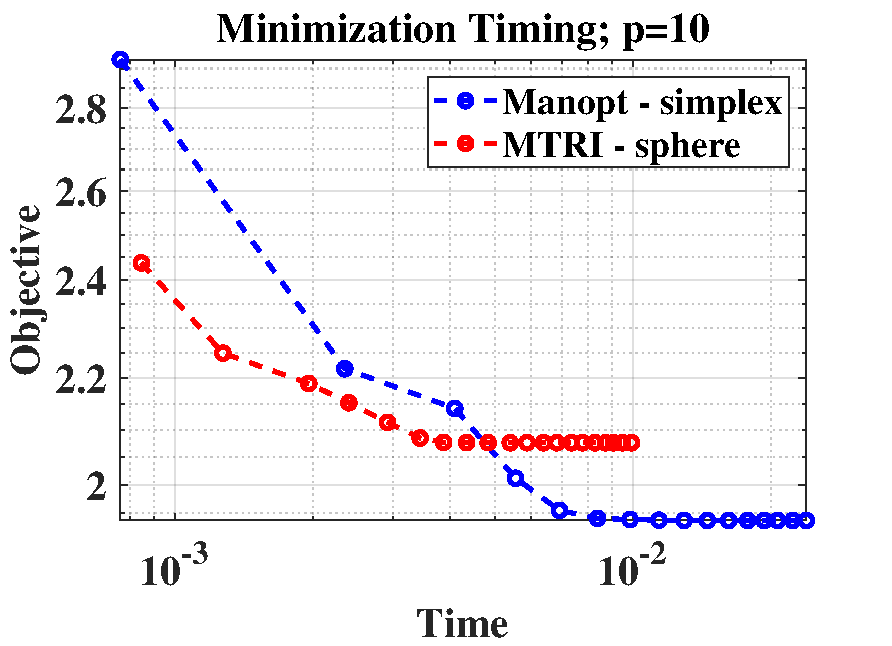
\includegraphics[scale = 0.4]{stuckSphericalMin.pdf}
	\caption{In this 10 dimensional minimization problem, the spherical minimizer gets stuck in $\alpha_7 = 0$ and is unable to correctly minimize the last 3 $\alpha$ values as $\nabla f(\alpha) \equiv 0$.}
\end{figure}

\subsection{Pad\'{e} Remapping Difficulties}

Though Pad\'{e} spline remapping has the potential to bring us out of the poorly conditioned regions of $\alpha$-space, it also has the potential to introduce "false optima". This is easily seen if $x_i \approx 0$, causing a flat region around the isometry point in that coordinate.

It seems imperative then that Pad\'{e} mappings are defined s.t. $T_i(y_\text{isom}) \tilde{\neq} \ 0$. However, this drawback makes the processes in \ref{contRemap}, \ref{kappaTrack} difficult and may require more thought

\begin{figure}[H]
	\centering
	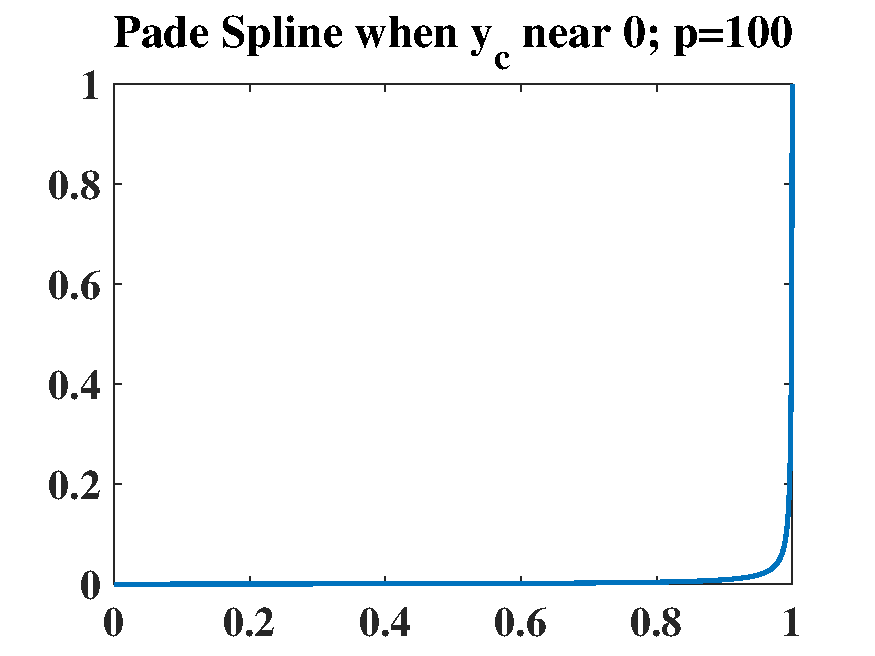
\includegraphics[scale=0.4]{pinnedPade.pdf}
	\caption{For a 100 dimensional problem, it is easy for a minimizer to run into $x_i \approx 0$, causing a Pad\'{e} mapping like above, causing stalling in the minimization and a near-zero gradient region after parametrization}
\end{figure}

\subsection{Condition Number Calculations}

As described in \ref{kappaTrack}, one can calculate the condition number of the Jacobian of the mapping from spherical coordinates onto the simplex. The properties of this mapping are partially determined by the Pad\'{e} splines determining $T(y_\text{isom})$. Here, we qualitatively investigate the properties of this conditioning by fixing a value of $T(y_\text{isom})$ and sweeping along a 1D slice of $\mathcal{S}_3$ defined by $(x_1, \frac{1-x_1}{2}, \frac{1-x_1}{2})$. Note that the sphere-to-simplex point of isometry \big{(}$(\frac{1}{3},\frac{1}{3},\frac{1}{3})$\big{)} falls on this slice. \\

In the conditioning, we do see the expected problem, and an example of the remedied behavior. The condition number of our sphere-to-simplex transformation $M(\vec{\alpha})^2$ is low near the point of isometry, and increases moving away from it and towards the edge of $\mathcal{S}_3$. $M(\vec{\alpha})^2$ is non-differentiable on the boundary of the simplex and so we see the vertical asymptotes moving towards the edges.\\
Figure \ref{condFig} shows how the condition number in a region can be reduced through a Pad\'{e} reparametrization. The parameter space \textbf{y} becomes the shifted and squished parameter space \textbf{x} around $T(y_\text{isom})$.

\begin{figure}[H]
	\centering
	\subfloat{{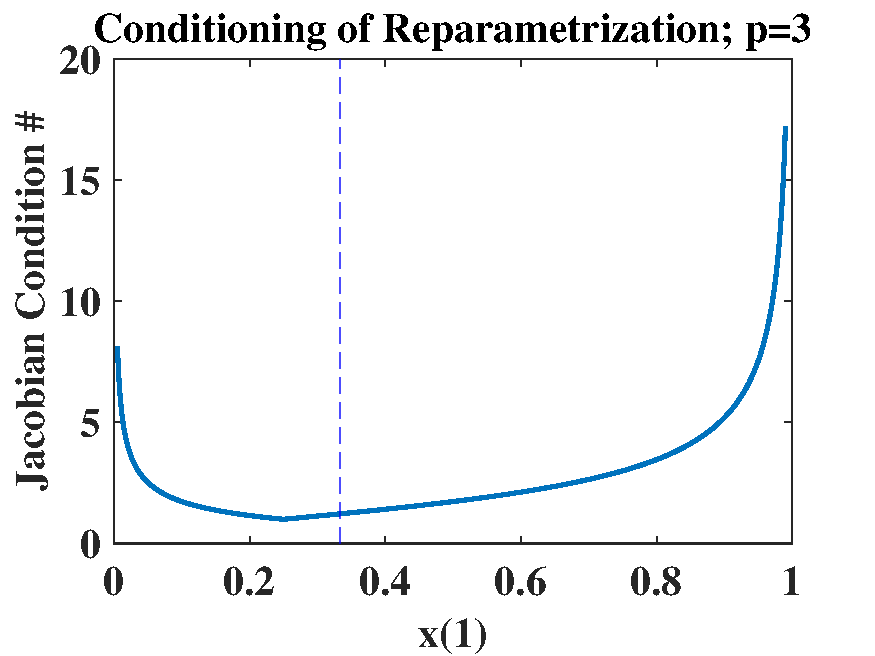
\includegraphics[width=5cm]{sphericalParamCond.pdf} }}%
	\qquad
	\subfloat{{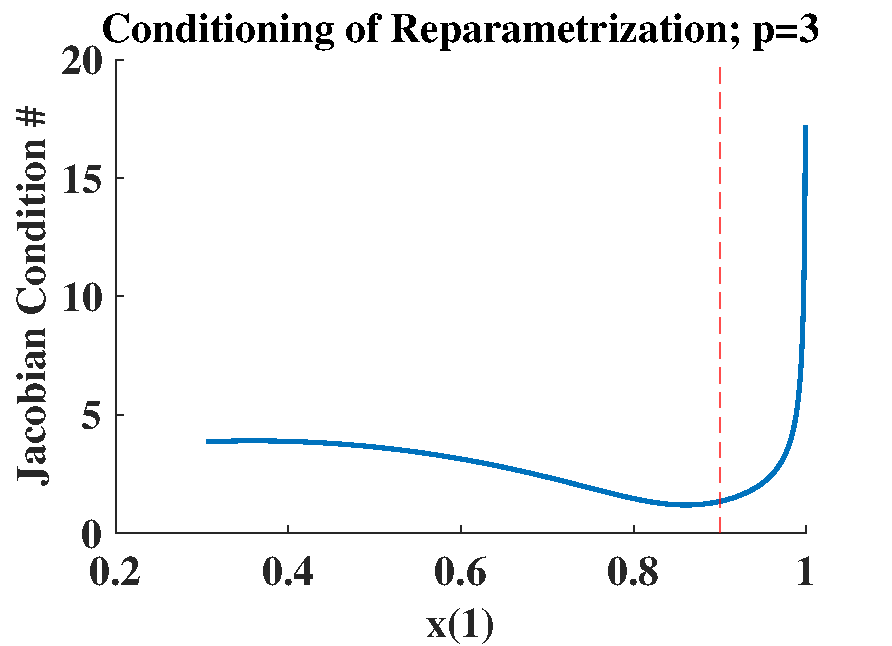
\includegraphics[width=5cm]{reparametrizedConditioning.pdf} }}%
	\caption{Condition number of the sphere-to-simplex Jacobian with no remapping (left). Condition number of the sphere-to-simplex Jacobian with a remapping s.t. $T(y_\text{isom}) = (0.95, 0.05, 0.05)$. Through the Pad\'{e} mapping we are able to reduce the condition number around our desired search location.}
	\label{condFig}
\end{figure}




\newpage 
\section{Current State/ To Do}

Currently I have an implementation of the method described in \ref{contRemap} using gradient descent, re-mapping after a set number of minimization steps. Here I detail notable next steps towards a better working routine.


\subsection{To Do:}

\begin{itemize}
	
	\item Find solution to Pad\'{e} ill-conditioning when $x_c, y_c \approx 0,1$
	\begin{itemize}
		\item Not so easy to say "stop remapping in these regions" as $x_0$ may easily end up in this region in at least one coordinate, ending remapping prematurely.
		
		\item A multidimensional spline (i.e. not coordinate-wise mapping) may be able to get around this problem
	\end{itemize}
	
	
	\item Implement spherical rotations to move non-differentiabilites out of minimization region.
	
\end{itemize}



\end{document}

